\documentclass[journal]{IEEEtran}
\usepackage[a5paper, margin=10mm, onecolumn]{geometry}
\usepackage[cmex10]{amsmath}
\usepackage{amssymb,amsfonts,amsthm}
\usepackage{gvv-book}
\usepackage{gvv}
\usepackage{hyperref}


\begin{document}
\title{7.4.32}
\author{EE25BTECH11025 - Ganachari Vishwambhar}
\maketitle

\textbf{Question}:\\
$ABCD$ is a square of side length 2 units. $C_1$ is the circle touching all the sides of the square $ABCD$ and $C_2$ is the circumcircle of square $ABCD$. $L$ is a fixed line in same plane and $\vec{R}$ is a fixed point.\\
\begin{enumerate}
    \item If $\vec{P}$ is any point of $C_1$ and $\vec{Q}$ is another point on $C_2$, then $\frac{PA^2+PB^2+PC^2+PD^2}{QA^2+QB^2+QC^2+QD^2}$
    \begin{enumerate}
    \begin{multicols}{4}
        \item 0.75
        \item 1.25
        \item 1
        \item 0.5
    \end{multicols}
    \end{enumerate}
    \item If a circle is such that it touches the line $L$ and the circle $C_1$ externally, such that both the circles are on the same side of the line, then locus of centre of the circle
    \begin{enumerate}
    \begin{multicols}{4}
        \item ellipse
        \item hyperbola
        \item parabola
        \item circle
    \end{multicols}
    \end{enumerate}
    \item A $L'$ through $\vec{A}$ is drawn parallel to $BD$. Point $S$ moves such that its distances from the line $BD$ and the vertex $\vec{A}$ are equal. If locus of $S$ cuts $L'$ at $T_2$ and $T_3$ and $AC$ at $T_1$, then area of $\triangle T_1T_2T_3$ is
    \begin{enumerate}
    \begin{multicols}{4}
        \item 1/2 sq.units
        \item 2/3 sq.units
        \item 1 sq.units
        \item 2 sq.units
    \end{multicols}
    \end{enumerate}
\end{enumerate}
\textbf{Solution: }\\
Let:\\
The centre of incircle and circumcircle be $\vec{O}$.\\
The radius of incircle be $r_1$ and that of circumcircle be $r_2$.\\
Given:
\begin{align}
    r_1 = 1\\
    r_2 = \sqrt{2}
\end{align}
\begin{enumerate}
\item Let $\vec{P}$ be any point on incircle and $\vec{Q}$ be any point on circumcircle.\\
$\vec{X}\epsilon \cbrak{\vec{A,B,C,D}}$
\begin{align}
    \norm{\vec{X}-\vec{P}}^2 = \norm{\vec{X}}^2 + \norm{\vec{P}}^2 - 2\vec{P}.\vec{X}\\
\end{align}
Summation over all $\vec{X}|\vec{X}\epsilon \cbrak{\vec{A,B,C,D}}$:
\begin{align}
    \sum \norm{\vec{X}-\vec{P}}^2 = \sum \norm{\vec{X}}^2 + 4.\norm{\vec{P}}^2 -2\vec{P}\sum \vec{X}\\
\end{align}
For, $\vec{P}$ = $\vec{P}$
\begin{align}
    \sum \norm{\vec{X}-\vec{P}}^2 = \sum \norm{\vec{X}}^2 + 4.\norm{\vec{P}}^2 -2\vec{P}\sum \vec{X}\\
    4\brak{1^2+1^2} + 4\brak{1}-2\vec{P}\brak{\myvec{1\\1}+\myvec{1\\-1}+\myvec{-1\\1}+\myvec{-1\\-1}}\\
    \therefore \norm{\vec{A}-\vec{P}}^2+\norm{\vec{B}-\vec{P}}^2+\norm{\vec{C}-\vec{P}}^2+\norm{\vec{D}-\vec{P}}^2 = 12
\end{align}
For, $\vec{P}$ = $\vec{Q}$
\begin{align}
    \sum \norm{\vec{X}-\vec{Q}}^2 = \sum \norm{\vec{X}}^2 + 4.\norm{\vec{Q}}^2 -2\vec{Q}\sum \vec{X}\\
    4\brak{1^2+1^2} + 4\brak{2}-2\vec{Q}\brak{\myvec{1\\1}+\myvec{1\\-1}+\myvec{-1\\1}+\myvec{-1\\-1}}\\
    \therefore \norm{\vec{A}-\vec{Q}}^2+\norm{\vec{B}-\vec{Q}}^2+|\norm{\vec{C}-\vec{Q}}^2+norm{\vec{D}-\vec{Q}}^2 = 12
\end{align}
conclusion:
\begin{align}
    \frac{12}{16}=0.75
\end{align}
Hence, option(a) is correct.

\item Let the radius of the moving circle be $r$, the centre of the circle be $\vec{X}$ and the line equation be $\vec{\hat{n}}^\top\vec{X}=c$,
\begin{align}
    |\vec{\hat{n}}^\top\vec{X}-c|=r\\
    ||\vec{X}||=r+1\\
    ||\vec{X}||=|\vec{\hat{n}}\vec{X}-\brak{c-1}|\\
    ||\vec{X}||^2=|\vec{\hat{n}}\vec{X}-\brak{c-1}|^2\\
    \vec{X}^\top\vec{X}=\brak{\vec{\hat{n}^\top\vec{X}}}^2+\brak{c-1}^2-2\vec{\hat{n}}^\top\vec{X}\brak{c-1}\\
    \vec{X}^\top\vec{X}-\brak{\vec{\hat{n}}\vec{X}}^2+2\vec{\hat{n}^\top\vec{X}}\brak{c-1}-\brak{c-1}^2\\
    \vec{X}^\top\brak{I-\vec{\hat{n}}\vec{\hat{n}}^\top}\vec{X}+2\brak{c-1}\vec{\hat{n}^\top\vec{X}}-\brak{c-1}^2
\end{align}
Equation (20) is the equation of parabola.\\
Hence, correct option is (c).

\item Let the point moving point be $S$ and the line equation be $\vec{n}^\top\vec{S}=0$.
\begin{align}
    \frac{|\vec{n}^\top\vec{S}|}{||\vec{n}||}=||\vec{S}-\vec{A}||\\
    \frac{|\vec{n}^\top\vec{S}|^2}{||\vec{n}||^2}=||\vec{S}-\vec{A}||^2\\
    \frac{|\vec{S}^\top\vec{n}\vec{n}^\top\vec{S}|}{||\vec{n}||}=\brak{\vec{S}-\vec{A}}^\top\brak{\vec{S}-\vec{A}}\\
    \vec{S}^\top\brak{I-\vec{\hat{n}}\vec{\hat{n}}^\top}\vec{S}-2\vec{A}^\top\vec{S}+\vec{A}^\top\vec{A}=0
\end{align}
Equation 24 is the locus of the moving point.\\
Let:
\begin{align}
    \vec{A}=\myvec{1\\1};\vec{B}=\myvec{-1\\1}\\
    \vec{C}=\myvec{-1\\-1};\vec{D}=\myvec{1\\-1}
\end{align}
$\vec{m_1}$ be the direction vector of line AC, $\vec{m_2}$ be the direction vector of line $L'$.
\begin{align}
    \vec{m_1} = \myvec{-2\\-2}=\myvec{1\\1}\\
    \vec{m_2} = \myvec{2\\-2}
\end{align}
The equation of line $L'$ 
\begin{align} \vec{S}=\vec{A}+t\vec{m_2}\end{align}
The equation of the line AC
\begin{align}
\vec{S}=\lambda \vec{m_1}
\end{align}
Substituting equation (30) in (24) we get $\lambda=\frac{1}{2}$:
\begin{align}
    \vec{T_1}=\frac{1}{2}\myvec{1\\1}
\end{align}
Substituting (29) in (24) we get $t=\frac{-1}{2},\frac{1}{2}$
\begin{align}
    \vec{T_2}=\myvec{0\\2}\\
    \vec{T_3}=\myvec{2\\0}
\end{align}
Now, finding area of the triangle:
\begin{align}
    \triangle T_1T_2T_3=\frac{1}{2}\norm{\myvec{\vec{T_2}-\vec{T_1}&\vec{T_3}-\vec{T_2}}}\\
    \triangle T_1T_2T_3 = 1
\end{align}
Option (c) is correct.



\end{enumerate}

\begin{figure}[h!]
   \centering
   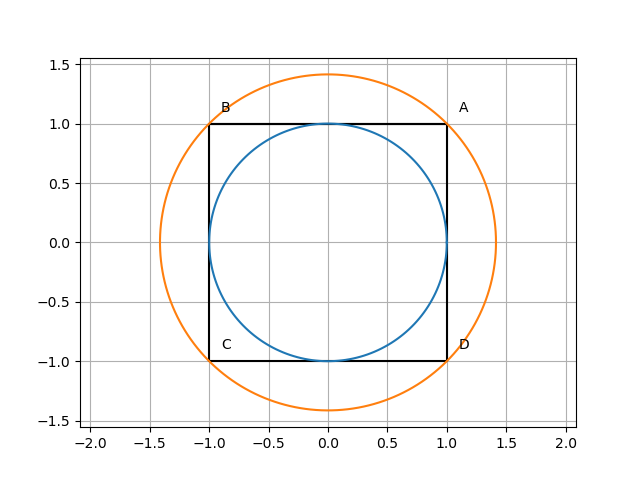
\includegraphics[width=0.7\linewidth]{figs/plot1.png}
   \caption{Plot of the given square and circles}
   \label{}
\end{figure}

\begin{figure}[h!]
   \centering
   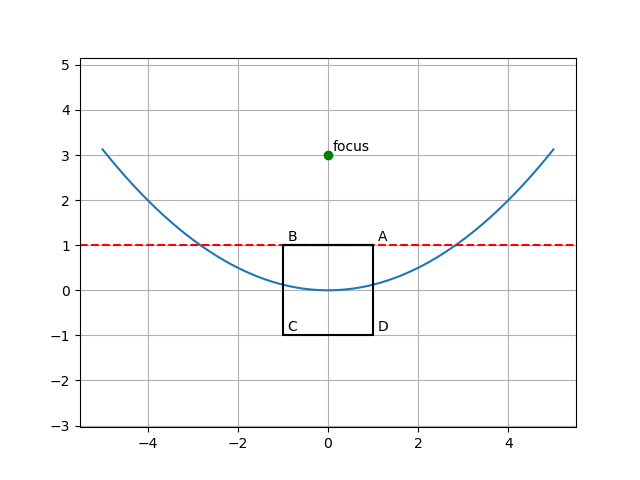
\includegraphics[width=0.7\linewidth]{figs/plot2.png}
   \caption{Plot of the given circles, square and locus of the point }
   \label{}
\end{figure}

\begin{figure}[h!]
   \centering
   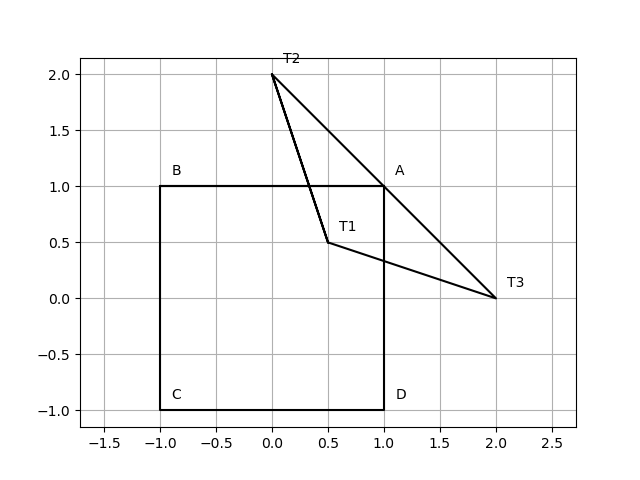
\includegraphics[width=0.7\linewidth]{figs/plot3.png}
   \caption{Plot of the given circles, square and locus of the point }
   \label{}
\end{figure}
\end{document}